\section{SHARED DESIGN CHOICES AND JOINT PERFORMANCE}
\label{sec:metrics}
\label{sec:tradeoffs}

A shared architecture becomes a performance question when a design variable
changes. Increasing pilot support can improve a reference while reducing the
data-bearing fraction; increasing probe power can strengthen sensing while
introducing interference; changing beam direction can alter both collected
power and the geometry available for estimation. The useful synthesis follows
the adjustable variable, the physical or processing mechanism, and the two
responses under the reported conditions. It also distinguishes a measured
response to a sweep from a modeled optimum or a proposed design relationship.

Figure~\ref{fig:coupling} summarizes this reasoning. The reviewed evidence
contains 402 substantive relationships from 168 studies, including quantitative
and qualitative descriptions. Their prevalence is reported in Electronic
Supplement S-Core; here, the emphasis is on how the mechanisms work.
Table~\ref{tab:metric_admissibility} provides selected within-study anchors.
Its rows illustrate different mechanisms and evidence forms rather than a
common performance ranking.

\begin{figure*}[t]
\centering
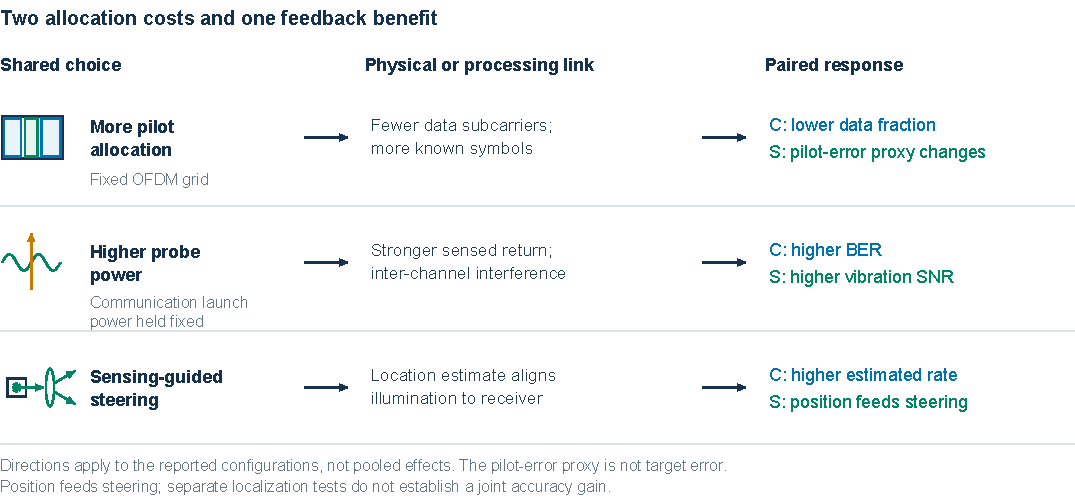
\includegraphics[width=\textwidth]{figures/coupling.pdf}
\caption{Two allocation costs and one feedback benefit in reported
configurations. More pilots occupy data subcarriers in a fixed OFDM grid;
the associated sensing measure is a pilot-error proxy
\cite{OISAC_SCR00007}. Higher probe power at fixed communication launch power
increases sensing SNR and BER \cite{OISAC_SCR00057}. A position estimate used
to steer illumination supports higher estimated communication rate
\cite{OISAC_SCR00196}; this does not imply a simultaneous improvement in
localization accuracy. Arrows explain these within-study mechanisms and do not
represent pooled trends.}
\label{fig:coupling}
\end{figure*}

\begin{table*}[t]
\caption{Selected mechanisms and their within-study performance evidence}
\label{tab:metric_admissibility}
\centering
\footnotesize
\setlength{\tabcolsep}{4pt}
\renewcommand{\arraystretch}{1.12}
\begin{tabularx}{\textwidth}{@{}>{\raggedright\arraybackslash}p{0.19\textwidth}
>{\raggedright\arraybackslash}p{0.22\textwidth}
>{\raggedright\arraybackslash}p{0.22\textwidth}
>{\raggedright\arraybackslash}X@{}}
\toprule
Shared choice & Communication response & Sensing response & Interpretation
conditions and evidence \\
\midrule
Embedded pilot allocation \cite{OISAC_SCR00007} & Changes BER and the data
subcarrier fraction & More pilot support improves the reported pilot-deviation
proxy & Simulation; known-pilot error is the reported sensing measure. The
data fraction and cyclic-prefix overhead are defined separately. \\
Probe-to-telecom power ratio \cite{OISAC_SCR00057} & Higher ratio raises BER;
the strongest penalty occurs near the probe & Higher ratio improves sensing
SNR & Fiber probe sweep at fixed communication launch power; retain probe
location and receiver conditions. \\
Sequence-transition shaping \cite{OISAC_SCR00052} & Reduces the communication
penalty from nonlinear interference & Retains phase sensing at the reported
condition & Shared fiber link with coherent reflectometry; the control changes
how interference is generated. \\
Waveform direct-current (DC) offset \cite{OISAC_SCR00808} & Error vector
magnitude (EVM) rises as the sensing component
is strengthened & Radar signal-to-interference ratio rises & Millimeter wave
waveform; energy redistribution changes the two recovery conditions. Higher
EVM indicates worse communication signal quality. \\
Camera exposure time \cite{OISAC_SCR00273} & Exposure is part of the modeled
communication/coexistence design & Exposure also governs the modeled sensing
response & Analytical and numerical coexistence; laboratory gains for the two
functions came from separate configurations. \\
Precoding and photodiode orientation \cite{OISAC_SCR00940} & Communication
quality is constrained above a stated threshold & Sensing contrast is
maximized within that feasible region & Optical phased array simulation;
emitter power, scene, orientation, and metric definitions constrain the
solution. \\
Source and carrier-recovery design \cite{OISAC_SCR01070} & Coherent data are
recovered using broad-linewidth lasers & Vibration is recovered through
residual-carrier processing & Long-span fiber experiment; hardware reuse moves
requirements into phase recovery and digital processing, without a universal
cost ranking. \\
\bottomrule
\end{tabularx}
\end{table*}

\subsection{Allocating Signal Space and Observation Time}

When communication and sensing occupy a finite frame, an allocation changes
both the samples available to the estimator and the opportunity to carry
payload. Embedded-pilot OFDM makes this connection explicit. Increasing pilot
support improves the reported pilot-deviation proxy, while BER and the data
subcarrier fraction follow the selected allocation
\cite{OISAC_SCR00007}. That proxy describes errors in known pilot symbols in a
simulated channel; it does not establish target range or localization accuracy.
The study's spectral-efficiency definition counts data subcarriers and treats
cyclic-prefix overhead separately. Thus, the same allocation informs three
reported outcomes, but each retains a different meaning.

Reserved intervals, subbands, and chirps extend the mechanism to other
waveforms. Protection can isolate a sensing return, and a chirp can supply
pulse-compression support, at the cost of occupying a particular part of the
available signal space \cite{OISAC_SCR00344,OISAC_SCR00366}. In a photonic
terahertz prototype, net communication rates depend on subcarrier assignment,
payload occupancy, and coding overhead \cite{OISAC_SCR01054}. The resource
cost therefore follows from the implemented frame, including the information
needed for synchronization and recovery. It cannot be inferred from the
modulation order or nominal bandwidth alone.

Full waveform reuse changes this accounting: sensing can use samples that also
carry data, but the receiver must recover a reference or separate the two
signal components. Full-grid OFDM reuse and shared optical waveforms illustrate
this alternative \cite{OISAC_SCR00274,OISAC_SCR01115}. A wider usable
bandwidth can support communication signaling and finer delay discrimination
at the same time. The benefit is limited by the device response, reference
quality, sidelobes, and receiver processing
\cite{OISAC_SCR00965,OISAC_SCR00988,OISAC_SCR01000}. A bandwidth ratio is
therefore informative only with the total bandwidth, target range, and
receiver architecture \cite{OISAC_SCR00784}.

Observation time creates a related, but distinct, allocation. Camera exposure,
acquisition duration, and task scheduling affect sensing support and update
cadence alongside data recovery or execution time
\cite{OISAC_SCR00189,OISAC_SCR00273,OISAC_SCR00833}. Longer observation does
not merely consume a frame fraction: it can change which temporal variations
remain observable. Chirp repetition, coding traffic, and embedded pulse count
likewise place the two functions in a common schedule
\cite{OISAC_SCR01015,OISAC_SCR01034,OISAC_SCR01019}. The exposure-time
coexistence analysis in Table~\ref{tab:metric_admissibility} is especially
instructive because the modeled shared choice and the separately obtained
laboratory gains support different conclusions \cite{OISAC_SCR00273}.

\subsection{Distributing Power Under Interference and Receiver Limits}

Power enters the joint design through a reference plane and a constraint.
Changing a probe-to-data ratio at fixed communication launch power adds a
different burden from dividing a fixed total budget. Launch power, received
power, carrier-to-signal ratio, modulation swing, and detector bias refer to
different points in the chain. Their effects pass through loss, noise,
nonlinear interaction, and saturation before either functional metric is
formed. Consequently, a reported gain can be interpreted only after identifying
what power was varied and what remained fixed.

The fiber probe sweep in Table~\ref{tab:metric_admissibility} exhibits a direct
conflict. Raising the sensing-to-telecom ratio at fixed communication launch
power improves sensing SNR and raises BER, with the strongest communication
penalty near the probe \cite{OISAC_SCR00057}. Related fiber designs connect
probe or carrier ratios to phase, polarization, and vibration observability
under their own OSNR and receiver conditions
\cite{OISAC_SCR00013,OISAC_SCR00072,OISAC_SCR00220}. These observations locate
the interaction in the optical link; they do not justify transferring a
preferred ratio between different fiber topologies or receivers.

Architecture determines where that power is spent. Polarization paths, receiver
taps, and separate service branches distribute the signal before estimation
\cite{OISAC_SCR00346,OISAC_SCR01072,OISAC_SCR01075}. In a visible-light
prototype, allocation between a communication/ranging branch and an
energy-harvesting branch governs their reported outcomes under distinct
receiver and endpoint bias conditions \cite{OISAC_SCR01025}. In photonic
wireless systems, carrier and waveform ratios interact with phase recovery and
the headroom available for communication and radar reception
\cite{OISAC_SCR00492,OISAC_SCR00954,OISAC_SCR00966}. The same allocation can
therefore produce different responses after a change in receiver architecture.

Absolute-power and drive sweeps expose another limit. Fiber launch conditions
affect nonlinear interaction and sensing reach
\cite{OISAC_SCR00473,OISAC_SCR01079,OISAC_SCR01180}; photonic front ends add
modulator, converter, and amplifier limits
\cite{OISAC_SCR00631,OISAC_SCR00986,OISAC_SCR01012}. Once a component limits
recovery, additional signal power need not provide proportional improvement.
Loss, pointing, and branch insertion loss also determine the margin actually
available at the detector \cite{OISAC_SCR00002,OISAC_SCR00218,OISAC_SCR00506}.
The useful operating region is bounded by these physical limits and by the
communication and sensing thresholds required together.

\subsection{Choosing Geometry, Aperture, and Spatial Support}

Spatial design changes both received energy and the information carried by the
available paths. Directing more light toward a communication receiver can
increase its signal, while sensing also depends on the positions and angles
needed to distinguish a target or estimate a location. Beam steering, access
point placement, and spatial allocation therefore influence coverage and
observability through related but unequal mechanisms
\cite{OISAC_SCR00036,OISAC_SCR00527,OISAC_SCR00914}. A common physical path
does not by itself imply that the communication receiver and sensing target
favor the same beam.

Joint optimization expresses this dependence through an explicit feasible
region. In the optical phased array simulation in
Table~\ref{tab:metric_admissibility}, precoding and photodiode orientation are
selected to maximize sensing contrast while satisfying a communication quality
threshold and emitter power constraints \cite{OISAC_SCR00940}. The result
establishes performance under the modeled scene and constraints. A related
spatial design shows communication gain and target-profile estimation
benefiting under alignment conditions \cite{OISAC_SCR00941}. Such joint gains
are plausible when the useful spatial support overlaps; the stated geometry is
part of the explanation, rather than an incidental test detail.

Geometry also enters through feedback. Structured illumination can provide a
position estimate used to adapt communication beamforming
\cite{OISAC_SCR00196}. Blockage-aware access can select a different usable
path \cite{OISAC_SCR01011}. The control decision may improve the subsequent
link, but its benefit depends on whether the observation remains current when
the action occurs. This creates a bridge from static spatial optimization to
the service timing examined in Section~\ref{sec:technologies_applications_6g}.

Spatial claims must also retain the implemented receiver configuration. Source
directivity and tag-delay spacing affect coverage and the separability of
returns \cite{OISAC_SCR01024,OISAC_SCR01050}. In another prototype, four
surrounding receivers were designed but one was operated
\cite{OISAC_SCR00619}. The measured configuration supports conclusions about
that receiver path; array-wide coverage and crosstalk require their own tests.

\subsection{Designing Waveforms and Recovering Shared Information}

Waveform design can change the origin of interference as well as the allocation
of signal energy. This distinction explains why superficially similar metric
pairs exhibit different trends. In fiber communication with coherent
reflectometry, shaping sequence transitions reduces nonlinear interference,
lowering the communication penalty while retaining phase sensing at the
reported condition \cite{OISAC_SCR00052}. A millimeter wave design instead
increases a DC offset to strengthen the sensing component: radar
signal-to-interference ratio improves while communication EVM rises
\cite{OISAC_SCR00808}. The former modifies the interference mechanism; the
latter changes the balance of energy within the waveform.

Sequence timing governs another set of coupled outcomes. Code length and
period can connect signaling rate with delay resolution and unambiguous range
\cite{OISAC_SCR00896,OISAC_SCR00576}. Chip duration, amplitude-keying timing,
and guard duration likewise determine the signal support for data recovery and
range discrimination \cite{OISAC_SCR00387,OISAC_SCR00887,OISAC_SCR00913}.
Embedding communication data into a sensing signal can change its correlation
or distributed-sensing fidelity \cite{OISAC_SCR00647,OISAC_SCR00918}.
Reported rate--range relations therefore require the precise timing and
ambiguity definitions; resolution, estimation error, and maximum unambiguous
range remain different outcomes.

Receiver processing can also reuse information obtained by the other function.
In the fiber probe study, a communication-receiver estimate of the link
frequency response is used to pre-compensate the sensing probe, improving
vibration-spectrum SNR by 2.4~dB in that processing test
\cite{OISAC_SCR00057}. This result concerns compensation using shared receiver
information; it is separate from the probe-power sweep and its communication
penalty.

Receiver processing also decides how the acquired samples become estimates. Spectral
weighting and transform choices alter the recovered response and computational
burden under a stated acquisition window
\cite{OISAC_SCR00998,OISAC_SCR01018,OISAC_SCR01095}. Zero padding refines the
sampled transform grid; it does not add independent delay information or,
by itself, improve the physical separability set by the acquired signal.
Similarly, changing a sensing estimator alone does not establish a joint
communication--sensing improvement. Kalman tuning acts within the sensing
branch \cite{OISAC_SCR00665}, whereas loss weighting in a joint inference
design explicitly connects communication reliability with distance and velocity
errors \cite{OISAC_SCR00233}. The metric and branch affected by the processing
change must therefore remain visible.

Source and digital processing choices can exchange implementation burden. One
terahertz design uses coherent comb generation to stabilize quadrature
phase-shift keying (QPSK) and LFM paths
\cite{OISAC_SCR01000}. A long-span fiber experiment recovers coherent data and
vibration using broad-linewidth lasers and residual-carrier processing
\cite{OISAC_SCR01070}. These examples place reference recovery in different
parts of the chain. They support architecture-specific feasibility, while a
cost or energy comparison would require matched hardware, processing, and
performance assumptions.

The processing burden also has a time dimension. Receiver bandwidth, converter
rate, memory, and acquisition length determine how quickly a result is
available. The outdoor terahertz study reports pipeline latency through
hardware analysis and communication/ranging performance through a field
experiment \cite{OISAC_SCR01054}. A smartphone camera system evaluates
recognition and communication in the laboratory and module latency, memory,
and complete-cycle timing on the device \cite{OISAC_SCR00833}. These
measurements describe complementary parts of the implementation; their
endpoints must align before they constitute an end-to-end latency result.

\subsection{What the Reported Operating Points Establish}

The mechanisms above explain both conflict and shared benefit. Allocating a
finite resource can favor one task at the expense of another. Suppressing a
common impairment or aligning useful spatial support can instead improve the
conditions for both. A source-reported parameter sweep, a constrained model,
and two separate demonstrations establish different parts of that argument.
In particular, a modeled optimum remains conditional on its objective,
constraints, noise model, and geometry; it is not a measured frontier for all
systems using the same platform.

The comparison conditions in Section~\ref{sec:foundations_comparison} determine
whether the magnitude of a response can inform another design. Where those
conditions differ, the transferable insight is the mechanism and the constraint
that limits it. The remaining question is whether that explanation survives
physical disturbances and can be tested independently.
Section~\ref{sec:validation_reproducibility} examines the corresponding
validation evidence.
